\documentclass{article}

\title{Introduction to Modern C++ Quiz 1}
\author{Ryan Baker}
\date{\today}

\usepackage[dvipsnames]{xcolor}
\usepackage{listings}
\usepackage{amsmath}
\usepackage{tikz}

\definecolor{JadeGreen}{RGB}{91,158,62}
\lstdefinestyle{catppuccin}{
	backgroundcolor=\color{White},
	commentstyle=\color{Gray},
	numberstyle=\footnotesize\ttfamily\color{Gray},
	stringstyle=\color{JadeGreen},
	keywordstyle=\color{BurntOrange},
	basicstyle=\ttfamily\footnotesize\color{Black},
	breakatwhitespace=false,
	breaklines=true,
	captionpos=b,
	keepspaces=true,
	numbers=left,
	numbersep=5pt,
	showspaces=false,
	showstringspaces=false,
	showtabs=false,
	tabsize=4,
}
\lstset{style=catppuccin}

\begin{document}

\maketitle

\begin{enumerate}
	\item What is the purpose of the \texttt{main} function?
	\begin{itemize}
		\item[a)] Declares global variables to be used by all files in the project
		\item[b)] {Serves as the entry point where program execution begins}
		\item[c)] It controls the flow of the compilation and linking process
		\item[d)] The function ``\texttt{main}'' has no special purpose
	\end{itemize}
	\vspace{1em}
	\item Which does the preprocessor \textbf{NOT} do in the C++ build process?
	\begin{itemize}
		\item[a)] Performs text replacement using \textcolor{BurntOrange}{\texttt{\#define}}
		\item[b)] Copies and pastes files using \textcolor{BurntOrange}{\texttt{\#include}}
		\item[c)] Conditionally compiles code with \textcolor{BurntOrange}{\texttt{\#if}}, \textcolor{BurntOrange}{\texttt{\#ifdef}}, and \textcolor{BurntOrange}{\texttt{\#ifndef}}
		\item[d)] {Translates C++ code into machine code}
	\end{itemize}
	\vspace{1em}
	\item Match each stage of the C++ build process with its output file type:
	\begin{center}{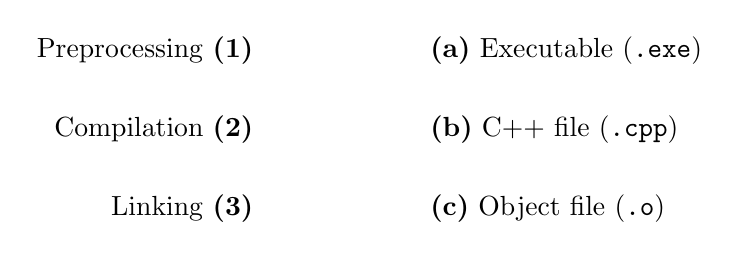
\begin{tikzpicture}
		\draw
		(0,2) node[left]  {Preprocessing \textbf{(1)}}
		(0,1) node[left]  {Compilation \textbf{(2)}}
		(0,0) node[left]  {Linking \textbf{(3)}}
		(2,2) node[right] {\textbf{(a)} Executable (\texttt{.exe})}
		(2,1) node[right] {\textbf{(b)} C++ file (\texttt{.cpp})}
		(2,0) node[right] {\textbf{(c)} Object file (\texttt{.o})}
		;
	\end{tikzpicture}}\end{center}
	\item Which of the following accuratley describes a ``translation unit''?
	\begin{itemize}
		\item[a)] {A \texttt{.cpp} file, plus the content of any files \textcolor{BurntOrange}{\texttt{\#include}}d}
		\item[b)] A single object file output by the compiler
		\item[c)] A chunk of code that the compiler translates into machine code
		\item[d)] The final executable file after the linking process
	\end{itemize}
	\vspace{1em}
	\item You attempt to build your C++ project with your favorite compiler and see the following message:
	\lstinputlisting[]{lderror.txt}
	\noindent
	Which type of error is this?
	\begin{itemize}
		\item[a)] Compilation error
		\item[b)] {Linking error}
		\item[c)] Runtime error
	\end{itemize}
	\vspace{1em}
	\item Given the following code: \lstinputlisting[language=C++]{unit.cpp}		
	the associated translation unit will include which of the following? \textbf{(select all that apply)}
	\begin{itemize}
		\item[a)] {The contents of \texttt{vector}}
		\item[b)] {The contents of \texttt{chrono}}
		\item[c)] {The source code in \texttt{regex.hpp}}
		\item[d)] The source code in \texttt{regex.cpp}
		\item[e)] The integer \texttt{MAX\_ITER} = 1000
		\item[f)] {The integer \texttt{FORCEINLINE} = 1}
		\item[g)] The integer \texttt{STATUS} = 2
		\item[h)] {The function \texttt{main}}
		\item[i)] The comment \textcolor{Gray}{\texttt{// do something}}
	\end{itemize}
	\pagebreak
	\item What is the output of this code:
	\lstinputlisting[language=C++]{sizeof.cpp}
	\begin{itemize}
		\item[a)] \texttt{1, 2, 3, 4}
		\item[b)] {\texttt{1, 2, 4, 8}}
		\item[c)] \texttt{2, 4, 8, 16}
		\item[d)] \texttt{8, 16, 32, 64} 
	\end{itemize}
	\item What is the maximum value representable by a \texttt{std::uint16\_t}? \begin{itemize}
		\item[a)] 32,767
		\item[b)] 32,768
		\item[c)] {65,535}
		\item[d)] 65,536
	\end{itemize}
\end{enumerate}

\end{document}